% Author: Seongjin Lee 
% Hanyang University, Seoul, Korea 
% esos.hanyang.ac.kr 
% 2016-09-11
% note: some slides are adopted from  \url{www.cs.stevens.edu/~jschauma/631A/}
% https://github.com/resourceful/lecture_sysprog/

\documentclass[newPxFont,sthlmFooter,nooffset]{beamer}
\usepackage{kotex}
%\usetheme{sthlm}
\usepackage{../beamer_template/beamerthemesthlm}
\hypersetup{pdfauthor={Seongjin Lee (insight@hanyang.ac.kr)},
            pdfsubject={Lecture Note: System Programming},
            pdfkeywords={Lecture Note, System Programming, class, undergraduate},
            pdfmoddate={D: \pdfdate},
            pdfcreator={Seongjin Lee}}

%\setbeamertemplate{footline}[text line]{%
%    \parbox{\linewidth}{\vspace*{-8pt} \insertsectionhead  \hfill\insertshortauthor\hfill\insertpagenumber}}
%\setbeamertemplate{navigation symbols}{}



\title{System Programming}
\subtitle{Week 3: File I/O}
\author[SJL]{Seongjin Lee}
\institute{\href{mailto:insight@hanyang.ac.kr}{insight@hanyang.ac.kr}\\\url{http://esos.hanyang.ac.kr}\\Esos Lab. Hanyang University}
\date{2016-09-21} 

\begin{document}



\frame[plain]{\titlepage} 

\frame{\frametitle{Table of contents}\tableofcontents} 


%---------------------------------------------------------
\section{File I/Os} 

\begin{frame}[t]{File Descriptors}
\begin{enumerate}[ ]
\item <1-> A {\em file descriptor} (or {\em file handle}) is a small, non-negative integer which identifies a file to the kernel.
\item <2-> Traditionally, \texttt{stdin}, \texttt{stdout} and \texttt{stderr} are 0, 1 and 2 respectively.
\item <3-> \hfill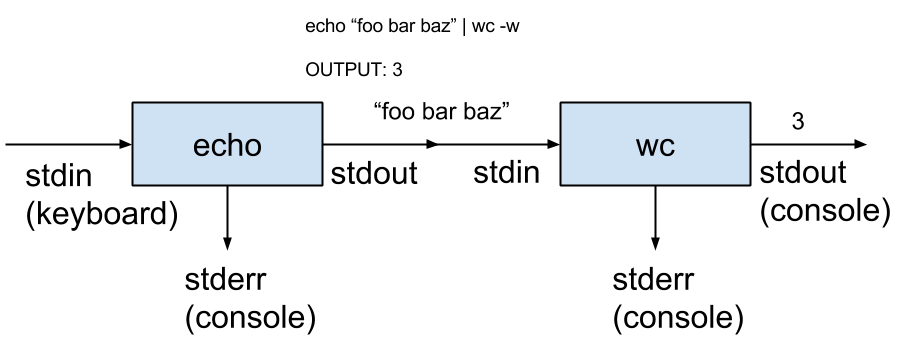
\includegraphics[width=0.7\linewidth]{./figure/stream-pipe.png}\hfill~
\item <4-> Relying on ``magic numbers'' is BAD.  Use \texttt{STDIN\_FILENO}, \texttt{STDOUT\_FILENO} and \texttt{STDERR\_FILENO} defined in <unistd.h> or \texttt{stdin}, \texttt{stdout}, and \texttt{stderr} defined in <stdio.h>.

\end{enumerate}
\end{frame}


\begin{frame}[t]{How many files can you open? (./codes/fdcount.c)}
\lstinputlisting[firstline=17,lineskip=-5pt]{./codes/fdcount.c}

How to compile \\
\texttt{\$ cd codes; cc -Wall -g -o fdcount fdcount.c}

\end{frame}


\subsection{Standard I/O}
\begin{frame}[t]{Basic File I/Os}
There are five fundamental \textsc{Unix} file I/O related functions: 
\begin{itemize}
	\item \texttt{open(2)}
	\item \texttt{close(2)}
	\item \texttt{lseek(2)}
	\item \texttt{read(2)}
	\item \texttt{write(2)}
\end{itemize}
\end{frame}

\begin{frame}[containsverbatim,t]{open(2)}

\begin{codedef}
#include <fcntl.h>
int open(const char *path, int oflag, ... /* mode_t mode */ );
int openat(int fd, const char *path, int oflag, ... /* mode_t mode */ );
\end{codedef}
Both return: file descriptor if OK, −1 on error
\bigskip

The \textit{path} parameter is the name of the file to open or create.
\bigskip

Options are specified by the \textit{oflag}
\end{frame}

\begin{frame}[t]{Options are}
\begin{columns}[t]
\begin{column}{0.30\linewidth}
\small \textit{oflag} must be one (and only one) of:
\footnotesize
\begin{itemize}
	\item \texttt{O\_RDONLY}\\ -- Open for reading only
	\item \texttt{O\_WRONLY}\\ -- Open for writing only
	\item \texttt{O\_RDWR}\\ -- Open for reading and writing
\end{itemize}
\end{column}
\begin{column}{0.70\linewidth}
\small and may be OR'd with any of these:
\footnotesize
\begin{itemize}
	\item \texttt{O\_APPEND} -- Append to end of file for each write
	\item \texttt{O\_CREAT} -- Create the file if it doesn't exist. Requires
		{\em mode} argument
	\item \texttt{O\_EXCL} -- Generate error if \texttt{O\_CREAT} and file
		already exists. (atomic)
	\item \texttt{O\_TRUNC} -- If file exists and successfully open in
		\texttt{O\_WRONLY} or \texttt{O\_RDWR}, make length = 0
	\item \texttt{O\_NOCTTY} -- If pathname refers to a terminal device, do
		not allocate the device as a controlling terminal
	\item \texttt{O\_NONBLOCK} -- If pathname refers to a FIFO, block special,
		or char special, set nonblocking mode (open and I/O)
	\item \texttt{O\_SYNC} --  Each write waits for physical I/O to complete
\end{itemize}
\end{column}
\end{columns}
\end{frame}


\begin{frame}[t]{openat(2)}
\texttt{openat(2)} function is equivalent to the open() function except in the case where the path specifies a relative path in an atomic fashion
\bigskip


\begin{itemize}
	\item \texttt{O\_EXEC} -- Open for execute only
	\item \texttt{O\_SEARCH} -- Open for search only (applies to directories)
	\item \texttt{O\_DIRECTORY} -- If path resolves to a non-directory file, fail and set errno to \texttt{ENOTDIR}.
	\item \texttt{O\_DSYNC} -- Wait for physical I/O for data, except
file attributes
	\item \texttt{O\_RSYNC} -- Block read operations on any pending writes.
	\item \texttt{O\_PATH} -- Obtain a file descriptor purely for fd-level operations. (Linux $>$2.6.36 only)
\end{itemize}
\end{frame}

\begin{frame}[containsverbatim,t]
  \frametitle{close(2)}

\begin{codedef}
#include <unistd.h> 
int close(int fd);   // Returns: 0 if OK, −1 on error
\end{codedef}

Closing a file releases any record locks that the process may have on the file. 


When a process terminates, all of its open files are closed automatically by the kernel. 
\bigskip

Many programs take advantage of this fact and don’t explicitly close open files. 
\bigskip



\end{frame}

\begin{frame}[containsverbatim,t]
  \frametitle{lseek example}

\texttt{cd ./codes ; make hole}

\begin{codedef}
James@maker:codes> make hole
cc -g -Wall -O0 -c hole.c
cc -g -Wall -O0 -o hole hole.o
James@maker:codes> ./hole
James@maker:codes> ls -l file.hole
-rw-------  1 James  staff  16394 Sep 15 23:46 file.hole
James@maker:codes> od -c file.hole
0000000     a    b    c    d    e    f    g    h    i    j  \0  \0  \0  \0  \0  \0
0000020   \0  \0  \0  \0  \0  \0  \0  \0  \0  \0  \0  \0  \0  \0  \0  \0
*
0040000    A   B   C   D   E   F   G   H   I   J
0040012
James@maker:codes>
\end{codedef}

\bigskip
Try making a file without a hole and compare the size of the two files.

\end{frame}

\begin{frame}[containsverbatim,t]
  \frametitle{creat(2)}

\begin{codedef}
#include <fcntl.h>
int creat(const char *path, mode_t mode);  \\ Returns: file descriptor opened for write-only if OK, −1 on error
\end{codedef}
\bigskip

it is equivalent to \texttt{open(path, O\_WRONLY | O\_CREAT | O\_TRUNC, mode);}
\bigskip

One deficiency with creat is that the file is opened only for writing.
\bigskip

If we were creating a temporary file that we wanted to write and then read back, we had to call creat, close, and then open. A better way is to use the open function, as in
\texttt{open(path, O\_RDWR | O\_CREAT | O\_TRUNC, mode);}

\end{frame}



\begin{frame}[containsverbatim,t]
  \frametitle{lseek(2)}
\begin{codedef}
#include <unistd.h>
off_t lseek(int fd, off_t offset, int whence);  \\ Returns: new file offset if OK, −1 on error
\end{codedef}
By default, this offset is initialized to 0 when a file is opened, unless the \texttt{O\_APPEND} option is specified.
\bigskip

The interpretation of the offset depends on the value of the whence argument.
\begin{itemize}
\item \texttt{SEEK\_SET} the file’s offset is set to offset bytes from the beginning of the file.
\item \texttt{SEEK\_CUR} the file’s offset is set to its current value plus the offset. The offset can be positive or negative.
\item \texttt{SEEK\_END} the  file’s offset is set to the size of the file plus the offset. The offset can be positive or negative.
\end{itemize}

\end{frame}



\begin{frame}[containsverbatim,t]
  \frametitle{read(2)}
\begin{codedef}
#include <unistd.h>
ssize_t read(int fd, void *buf, size_t nbytes); \\ Returns: number of bytes read, 0 if end of file, −1 on error
\end{codedef}  

There are several cases where \texttt{read} returns less than the number of bytes requested:
\begin{itemize}
\item \textbf{regular file:} EOF is reached before the requested number of bytes has been read. 
\item \textbf{terminal device:} Normally, up to one line is read at a time. 
\item \textbf{network: } Buffering within the network may cause less than the requested amount to be returned.
\item \textbf{a pipe or FIFO:} If the pipe contains fewer bytes than requested, read will return only what is available.
\item \textbf{interrupted by a signal} and a partial amount of data has already been read. 
\end{itemize}

\end{frame}



\begin{frame}[containsverbatim,t]
  \frametitle{write(2)}
\begin{codedef}
#include <unistd.h>
ssize_t write(int fd, const void *buf, size_t nbytes); \\ Returns: number of bytes written if OK, −1 on error
\end{codedef}  

The return value is usually equal to the nbytes argument; otherwise, an error has occurred. 
\begin{itemize}
  \item A common cause for a write error is either filling up a disk or exceeding the file size limit for a given process.
\end{itemize}
\bigskip

For a regular file, \texttt{write} starts at the file’s current offset. 
\bigskip

If the \texttt{O\_APPEND} option was specified when the file was opened, the file’s offset is set to the current end of file before each write operation. 
\bigskip

After a successful write, the file’s offset is incremented by the number of bytes actually written.
\end{frame}


\begin{frame}[containsverbatim,t]
  \frametitle{I/O Efficiency}
\lstinputlisting[lineskip=-5pt]{./codes/mycat.c}
\end{frame}

\begin{frame}[containsverbatim,t]
  \frametitle{I/O Efficiency cnt'd}
\begin{itemize}
\item  It reads from standard input and writes to standard output, assuming that these have been set up by the shell before this program is executed. Indeed, all normal UNIX system shells provide a way to open a file for reading on standard input and to create (or rewrite) a file on standard output. This prevents the program from having to open the input and output files, and allows the user to take advantage of the shell’s I/O redirection facilities.
\item The program doesn’t close the input file or output file. Instead, the program uses the feature of the UNIX kernel that closes all open file descriptors in a process when that process terminates.
\item This example works for both text files and binary files, since there is no difference between the two to the UNIX kernel.
\end{itemize}
\end{frame}


\begin{frame}[containsverbatim,t]
  \frametitle{I/O Efficiency cnt'd}
\texttt{cd codes; make iotest}
\bigskip

\lstinputlisting[linerange={17,30},lineskip=-5pt]{./codes/Makefile}
\end{frame}


\begin{frame}[t]
  \frametitle{I/O Efficiency cnt'd}
\centering
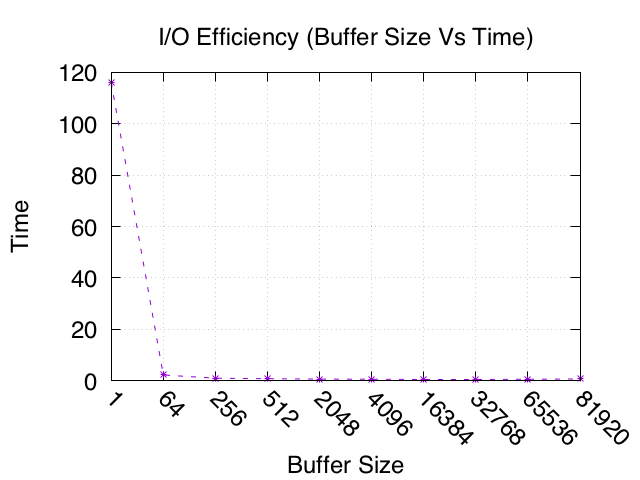
\includegraphics[width=0.85\linewidth]{./figure/iotest.png}
\end{frame}

\begin{frame}[t]
  \frametitle{I/O Efficiency cnt'd}
\centering
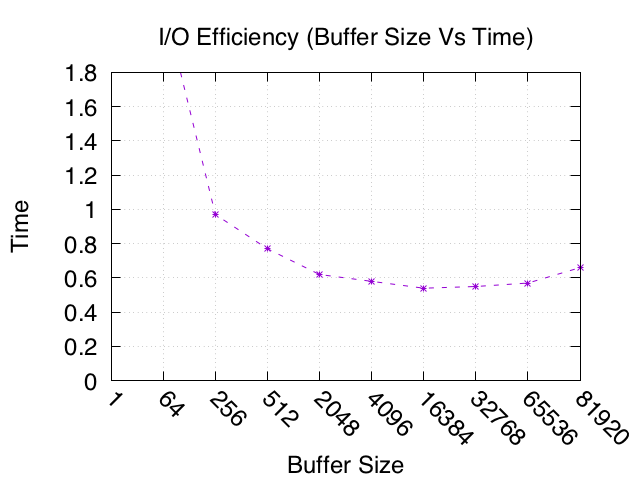
\includegraphics[width=0.85\linewidth]{./figure/iotest2.png}
\end{frame}


\section{File Sharing} 

\begin{frame}[t]{File Sharing}
Atomicity of the file fundamental file I/O functions
\bigskip

File sharing
\bigskip

manipulation of file descriptors
\end{frame}


\end{document}
